% The following TACC beamer style files must be in your TEXINPUTS path
% for this file to compile successfully:
% beamercolorthemeTACC.sty
% beamerfontthemeTACC.sty
% beamerinnerthemeTACC.sty
% beamerouterthemeTACC.sty
% beamerthemeTACC.sty
\documentclass
% [handout] % - doesn't work, just runs extra bullets off the bottom of the slide
{beamer}

%Drop the options in [] below if you don't like the stuff at the top of your slide.
% headernav gives the centered, side-by-side section/subsection headers
% headertree gives the expanding "tree" style section/subsection headers,
% and is based on beamerouterthemetree.sty.
% \usetheme[headernav]{TACC}
\usetheme[headertree]{TACC}
%\usetheme{TACC}

% A default Beamer theme
% /sw/share/texmf-dist/source/latex/beamer/themes/theme/beamerthemeAntibes.sty
% /sw/share/texmf-dist/tex/latex/beamer/beamerthemeAntibes.sty
%
% Antibes uses the following sub-themes
% \useoutertheme{tree}
% \usecolortheme{whale}
% \usecolortheme{orchid}
% \useinnertheme{rectangles}

%\usetheme{Antibes}


\usepackage{amsmath,amssymb,amsthm}
%\usepackage{graphicx} %% Uncomment if you're going to have figures
\usepackage{booktabs} % \toprule, \midrule, \bottomrule
% \usepackage{ulem} %\sout (use for creating strikeout text)
% \usepackage{tikz} % dia's LaTeX PGF macros export type.
                    % tikz pkg not installed by default

\usepackage{minted}

\newcommand{\comment}{\textcolor{defblockheader}}

% Macro for writing "C++" with closely-spaced "++"
\newcommand{\cpp}{C\nolinebreak\hspace{-.05em}\raisebox{.4ex}{\tiny\bf +}\nolinebreak\hspace{-.10em}\raisebox{.4ex}{\tiny\bf +}}

\title{Python in HPC}
\subtitle{Numpy, MatPlotLib, SciPy, and Cython}

% \event is only defined in the TACC theme
%\event{TACC 1-Day Training Series}

\author{Andy R. Terrel}
\institute{The Texas Advanced Computing Center}

% A record of dates when I've given the talk
\date{April 23, 2012}


% Turns on the use of rounded boxes with shadows
\setbeamertemplate{blocks}[rounded][shadow=true]

\begin{document}

\begin{frame}
  \titlepage
\end{frame}

\section*{Outline}% Make it easy to jump to this page in the PDF

% use outline_currentsection.tex to highlight the current section

% Auto-generate the TOC slide(s)
\begin{frame}
  %\tableofcontents[currentsection]
  \tableofcontents
\end{frame}



\section{Introduction}
% Auto-generate the TOC slide(s)
\begin{frame}
  \tableofcontents[currentsection, currentsubsection]
  %\tableofcontents
\end{frame}

\subsection*{Python philosophy}

\begin{frame}
  \begin{itemize}
  \item Beautiful is better than ugly.
  \item Explicit is better than implicit.
  \item Simple is better than complex.
  \item Complex is better than complicated.
  \item Flat is better than nested.
  \item Sparse is better than dense.
  \item Readability counts.
  \end{itemize}
\end{frame}

\begin{frame}
  \begin{itemize}
  \item Special cases aren't special enough to break the rules.
    \begin{itemize}
    \item Although practicality beats purity.
    \end{itemize}
  \item Errors should never pass silently.
    \begin{itemize}
    \item Unless explicitly silenced.
    \end{itemize}
  \item In the face of ambiguity, refuse the temptation to guess.
  \item There should be one-- and preferably only one --obvious way to do it.
    \begin{itemize}
    \item Although that way may not be obvious at first unless you're Dutch.
    \end{itemize}
  \end{itemize}
\end{frame}

\begin{frame}
  \begin{itemize}
    \item Now is better than never.
      \begin{itemize}
      \item Although never is often better than right now.
      \end{itemize}
    \item If the implementation is hard to explain, it's a bad idea.
    \item If the implementation is easy to explain, it may be a good idea.
    \item NameSpaces are one honking great idea -- let's do more of those!
  \end{itemize}
\end{frame}

%%   \begin{quotation}
%%     \noindent \cpp{} is just an abomination. Everything is wrong with it in every way.
%%   \end{quotation}
%%   \hspace{.6\textwidth}Jamie Zawinski \\
%%   \hspace{.6\textwidth}Netscape, 1994
%%   \vspace{.1\textheight}

%%   \begin{quotation}
%%     \noindent \cpp{} is a horrible language. It's made more horrible by the fact that a lot
%%     of substandard programmers use it \ldots
%% \end{quotation}
%%   \hspace{.6\textwidth}Linus Torvalds \\
%%   \hspace{.6\textwidth}Creator of Linux
%% \end{frame}


%% \begin{frame}
%%   \begin{quotation}
%%     \noindent \ldots by and large I think it's a bad language. It does
%% a lot of things half well and it's just a garbage heap of ideas that
%% are mutually exclusive. Everybody I know, whether it's personal or
%% corporate, selects a subset and these subsets are different.
%%   \end{quotation}
%% \hspace{.6\textwidth}Ken Thompson \\
%% \hspace{.6\textwidth}Google
%% \end{frame}



%% \begin{frame}
%% %  \begin{quotation}
%% %    \noindent There are two types of computer languages;
%% %    those that people hate, and those that nobody uses. \\
%% %  \end{quotation}
%% % \hspace{.6\textwidth}J.~K.~Ousterhout \\
%% % \hspace{.6\textwidth}Stanford University
%%   \begin{quotation}
%%     \noindent C makes it easy to shoot yourself in the foot; \cpp{} makes it harder,
%%     but when you do it blows your whole leg off.
%%   \end{quotation}
%%   \vspace{.1\textheight}
%%  \begin{quotation}
%%    \noindent There are only two kinds of [programming] languages: the
%%    ones people complain about, and the ones nobody uses.
%%  \end{quotation}
%%  \hspace{.6\textwidth}Bjarne Stroustrup \\
%%  %\hspace{.6\textwidth}Texas A\&M University \\
%%  \hspace{.6\textwidth}Creator of \cpp
%% \end{frame}

\subsection*{Facts about Python}

\begin{frame}
  Timeline
  \begin{itemize}\itemsep=.25cm
    \item{Began in 1989 at CWI as a successor of ``ABC''}
    \item{Initially developed by Guido van Rossum, now Benevolent Dictator for Life}
    \item{Primarily thought of initally as a teaching language}
    \item{Early release cylce every 6 months or so, currently every 2 years}
    \item{Currently core is moving to 3.0, but most libraries only work on 2.7}
  \end{itemize}
\end{frame}



\begin{frame}
  Technical Specifications
  \begin{itemize}\itemsep=.25cm
    \item{Python is a ``multi-paradigm'' language:
      \begin{itemize}
      \item{Imperative}
      \item{Object Oriented}
      \item{Dynamically Typed -- Interpreted}
      \item{Almost Functional}
      \end{itemize}
    }
  \item{This means that programmers can work in a variety of styles, freely
    intermixing constructs from different paradigms}
  \end{itemize}
\end{frame}

\begin{frame}
  Duck Typing
  \begin{itemize}
  \item If it looks like a duck, then it is a duck.
  \item Dynamically evaluates types
  \item Type (and name) errors not caught until runtime
    \begin{itemize}
    \item Unit testing becomes more important
    \item Good IDE can catch many standard errors
    \end{itemize}
  \end{itemize}
\end{frame}

\begin{frame}
  Speed
  \begin{itemize}
  \item Running Python code is usually 10X slower than C
  \item Writing Python code is usually much much much faster than writing C
  \item Reading Python code is usually much much much faster than reading C
  \item Write Python, profile, refine in C
  \item Several projects are working to speed up Python (PyPy, Cython, ...)
  \end{itemize}
\end{frame}

\begin{frame}
  Gotchas
  \begin{itemize}
  \item No multithreading support
  \item Import problem
  \end{itemize}
  But who cares, let's start hacking!
\end{frame}
%% \begin{frame}[fragile=singleslide]
%%   \begin{itemize}
%%   \item \cpp{} is often said to be a ``superset'' of C, but
%%   \end{itemize}
%% \vspace{.15in}
%%   \begin{equation}
%%     \nonumber
%%     \framebox{Superset of C}
%%     \nRightarrow
%%     % \fbox{any C code will compile with a \cpp{} compiler}
%%     \framebox{Any C code will compile with a \cpp{} compiler}
%%   \end{equation}
%%   \begin{itemize}
%%   \item{Simple example: \cpp{} introduces new keywords, so legal C code such as:
%%       \begin{columns}
%%         \column{.3\textwidth}
%%         \begin{block}{}
%% \begin{semiverbatim}
%% int class = 0;
%% int public = 0;
%% int private = 0;
%% int new = 0;
%% \end{semiverbatim}
%%       \end{block}
%% \end{columns}
%% %
%% \vspace{1ex}
%% will not compile with a \cpp{} compiler.
%%     }
%%   \end{itemize}
%% %   \framebox[.3\textwidth]{superset of C}
%% %   $\nRightarrow$
%% %   \framebox[.3\textwidth]{any C code will compile with a \cpp{} compiler}

%% %\begin{columns}[c]
%% %\column{.15\textwidth}
%% %Superset of C
%% %\column{.1\textwidth}
%% %$\nRightarrow$
%% %\column{.45\textwidth}
%% %Any C code will compile with a \cpp{} compiler
%% %\end{columns}
%% \end{frame}



%% \begin{frame}
%%   \begin{itemize}\itemsep=.75cm
%%   \item {Knowledge of C is \emph{absolutely not} required to begin programming in \cpp}
%%   \item {In fact, extensive C knowledge can be detrimental to learning \cpp{} because:
%%       \begin{itemize}
%%       \item{You already ``know'' how to do things in C, }
%%       \item{Therefore you are not exposed to the ``\cpp{} way'' of doing them }
%%       \item{Hence, you are still writing C code, but with a slower, more complicated
%%           compiler and worse binary compatibility!}
%%       \end{itemize}
%%     }
%%   \end{itemize}
%% \end{frame}



% LocalWords:  metaprogramming



\section{NumPy: Linear Algebra and Datastructures}
% Auto-generate the TOC slide(s)
\begin{frame}
  \tableofcontents[currentsection, currentsubsection]
  %\tableofcontents
\end{frame}

\subsection*{Numpy Introduction}

\begin{frame}[fragile]
How slow is Python?  Let's add one to a million numbers.

\begin{block}{Using lists}
\begin{minted}{python}
In [15]: lst = range(1000000)

In [16]: %timeit [i + 1 for i in lst]
10 loops, best of 3: 65.6 ms per loop
\end{minted}
\end{block}

\begin{block}{Using NumPy}
\begin{minted}{python}
In [18]: arr = arange(1000000)

In [19]: %timeit arr + 1
100 loops, best of 3: 2.91 ms per loop
\end{minted}
\end{block}
\end{frame}

\begin{frame}
  What makes an array so much faster?
  \begin{itemize}
  \item Data layout
    \begin{itemize}
    \item homogenous: every item takes up the same size block of memory
    \item single data-type objects
    \item powerful array scalar types
    \end{itemize}
  \item universal function (ufuncs)
    \begin{itemize}
    \item function that operates on ndarrays in an element-by-element fashion
    \item vectorized wrapper for a function
    \item built-in functions are implemented in compiled C code
    \end{itemize}
\end{itemize}
\end{frame}

\begin{frame}
  Data layout
  \begin{itemize}
  \item homogenous: every item takes up the same size block of memory
  \item single data-type objects
  \item powerful array scalar types
  \end{itemize}
  \begin{center}
    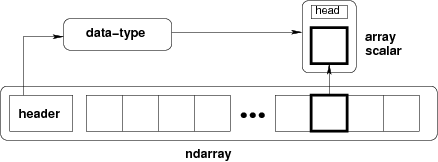
\includegraphics[scale=.5]{../figures/numpy/threefundamental.png}
  \end{center}
\end{frame}

\begin{frame}[fragile]
  universal function (ufuncs)
  \begin{itemize}
  \item function that operates on ndarrays in an element-by-element fashion
  \item vectorized wrapper for a function
  \item built-in functions are implemented in compiled C code
  \end{itemize}
  \begin{block}{python function v ufunc}
    \begin{minted}{python}
In [31]: %timeit [sin(i)**2 for i in arr]
1 loops, best of 3: 4.32 s per loop

In [32]: import numpy as np

In [33]: %timeit np.sin(arr)**2
10 loops, best of 3: 20.8 ms per loop
    \end{minted}
  \end{block}
\end{frame}


\subsection{Array slicing and striding}

\begin{frame}[fragile]
Finite Differences
 \begin{block}{computing blocks}
   \begin{minted}{python}
In [38]: x = np.arange(0, 20, 2)

In [40]: y = x**2

In [42]: dy_dx = ((y[1:] - y[:-1]) / (x[1:] - x[:-1]))
In [43]: dy_dx
Out[43]: array([ 2,  6, ... 30, 34])

In [44]: dy_dx_c = ((y[2:] - y[:-2])/(x[2:] - x[:-2]))
In [45]: dy_dx_c
Out[45]: array([ 4,  8, ... 28, 32])
\end{minted}
 \end{block}
\end{frame}



\subsection{Broadcasting}
\begin{frame}[fragile]
 Computing a 3D grid of distances $R_{ijk} = \sqrt(i^2 + j^2 + k^2)$
 \begin{block}{With temporary matrices}
   \begin{minted}{python}
In [44]: i, j, k = np.mgrid[-100:100, -100:100, -100:100]
In [45]: print(i.shape, j.shape, k.shape)
((200, 200, 200), (200, 200, 200), (200, 200, 200)

In [46]: R = np.sqrt(i**2 + j**2 + k**2)
In [47]: R.shape
Out[47]: (200, 200, 200)
\end{minted}
\end{block}
\end{frame}

\begin{frame}[fragile]
 Computing a 3D grid of distances $R_{ijk} = \sqrt(i^2 + j^2 + k^2)$
 \begin{block}{With temporary matrices}
   \begin{minted}{python}
# Construct the row vector that runs from -100 to +100
In [47]: i = np.arange(-100, 100).reshape(200, 1, 1)
#  Construct the column vector
In [48]: j = np.reshape(i, (1, 200, 1))
# Construct the depth vector
In [49]: k = np.reshape(i, (1, 1, 200))

In [50]: R = np.sqrt(i**2 + j**2 + ....: k**2)
In [51]: R.shape Out[49]: (200, 200, 200)
\end{minted}
 \end{block}
\end{frame}

\begin{frame}[fragile]
 Computing a 3D grid of distances $R_{ijk} = \sqrt(i^2 + j^2 + k^2)$
 \begin{center}
   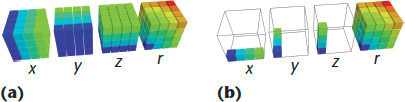
\includegraphics[scale=.5]{../figures/numpy/broadcasting.png}
 \end{center}
\end{frame}



\section{MatPlotLib: Easy Visualization}
% Auto-generate the TOC slide(s)
\begin{frame}
  \tableofcontents[currentsection, currentsubsection]
  %\tableofcontents
\end{frame}


\section{SciPy: Scientific toolkit}
% Auto-generate the TOC slide(s)
\begin{frame}
  \tableofcontents[currentsection, currentsubsection]
  %\tableofcontents
\end{frame}



\section{Cython: Speeding up to C speeds}
% Auto-generate the TOC slide(s)
\begin{frame}
  \tableofcontents[currentsection, currentsubsection]
  %\tableofcontents
\end{frame}


\section{Additional References}
% Auto-generate the TOC slide(s)
\begin{frame}
  \tableofcontents[currentsection, currentsubsection]
  %\tableofcontents
\end{frame}

%\input{cpp_further_reading}

\end{document}
